
\section{Database Model}

\begin{enumerate}
\def\labelenumi{\arabic{enumi}.}
\itemsep1pt\parskip0pt\parsep0pt
\item
  General Approach
\item
  Implementation
\end{enumerate}

\subsubsection{General Approach}\label{general-approach}

\begin{figure}[htbp]
\centering
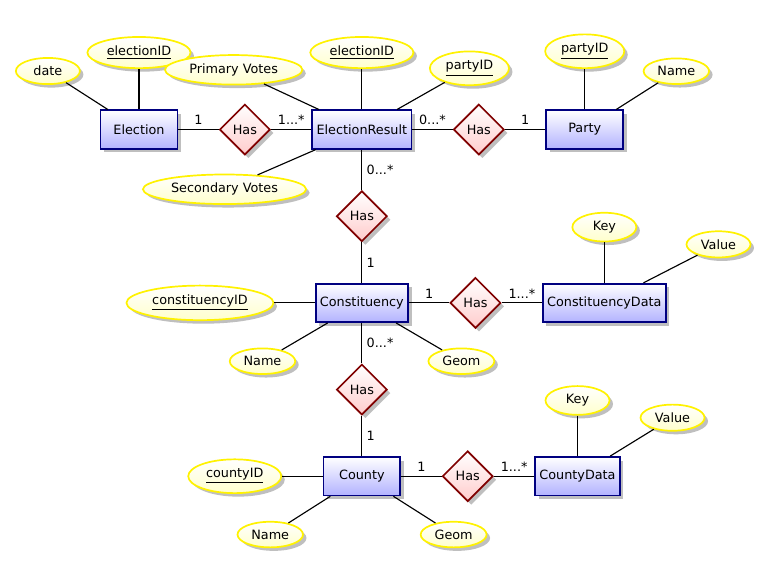
\includegraphics[width=1.1\textwidth]{../img/KIQu2J3.png}
\caption{uml}
\end{figure}

\subsubsection{Implementation}\label{implementation}

\textbf{Election Results}
\\Constituency 1\textless{}-\textgreater{}n
ElectionResult n\textless{}-\textgreater{}1
Party
\\ElectionResult(Constituency\_ID, Party\_ID, election\_ID,
primaryVotes, secondaryVotes)



\begin{lstlisting}
CREATE TABLE electionresult
(
  constituencyid integer NOT NULL,
  partyid integer NOT NULL,
  primaryVotes integer,
  secondaryVotes integer,
  election_electionid bigint,
  CONSTRAINT constituency_fk FOREIGN KEY (constituencyid)
      REFERENCES constituency (gid) MATCH SIMPLE
      ON UPDATE NO ACTION ON DELETE NO ACTION,
  CONSTRAINT election_fk FOREIGN KEY (election_electionid)
      REFERENCES election (electionid) MATCH SIMPLE
      ON UPDATE NO ACTION ON DELETE NO ACTION,
  CONSTRAINT party_fk FOREIGN KEY (partyid)
      REFERENCES party (partyid) MATCH SIMPLE
      ON UPDATE NO ACTION ON DELETE NO ACTION
)
\end{lstlisting}

\textbf{Party}
\\Party(Party\_ID, Name)


\begin{lstlisting}
CREATE TABLE party
(
  partyid serial NOT NULL,
  name character(200),
  color character varying(255),
  partyname character varying(255),
  CONSTRAINT party_pkey PRIMARY KEY (partyid)
)
\end{lstlisting}


\textbf{Election}
\\Election(election\_ID, date, year)
Election(election\_ID, date, year)

\begin{lstlisting}
CREATE TABLE election
(
  electionid bigint NOT NULL,
  date timestamp without time zone,
  year integer NOT NULL,
  CONSTRAINT election_pkey PRIMARY KEY (electionid)
)
\end{lstlisting}

\textbf{Constituency Data}
\\Constituency 1\textless{}-\textgreater{}n
ConstituencyData n \textless{}-\textgreater{} 1 ConstituencyDataKeys
ConstituencyData(Constituency\_ID, Key\_ID,
Value)\\ConstituencyDataKeys(Key\_ID, name)



\begin{lstlisting}
CREATE TABLE public.constituency_data
(
  gid BIGINT NOT NULL,
  key CHARACTER VARYING(255),
  value BIGINT NOT NULL,
  CONSTRAINT belongs_to_constituency FOREIGN KEY (gid)
      REFERENCES constituency (gid) MATCH SIMPLE
      ON UPDATE NO ACTION ON DELETE NO ACTION
)
\end{lstlisting}

\textbf{County Data}
\\County 1 \textless{}-\textgreater{} n CountyData n \textless{}-\textgreater{}
1 CountyDataKeys CountyData(County\_ID, Key\_ID, Value)
\\CountyDataKeys(Key\_ID, name)

\begin{lstlisting}
CREATE TABLE public.county_data
(
  gid BIGINT NOT NULL,
  key CHARACTER VARYING(255),
  value BIGINT NOT NULL,
  CONSTRAINT belongs_to_county FOREIGN KEY (gid)
      REFERENCES county (gid) MATCH SIMPLE
      ON UPDATE NO ACTION ON DELETE NO ACTION
)
\end{lstlisting}

\textbf{County}
\\County(County\_ID, Name, Nr, coordinates)

\textbf{Constituency}
\\Constituency(Constituency\_ID, Name, Nr,
coordinates)